\section{Tiny Tapeout 3}
\label{sec:tinytapeout3}

For Tiny Tapeout 3 the two clock buffers of Tiny Tapeout 1 and 2 were replaced by an inverting clock buffer design, with only one buffer between the clock input and output. Fig. ~\ref{fig:TT02_vs_TT03} shows a comparison between the TT02 and TT03 clock buffer designs. By inverting the clock between each design any asymmetry in the clock pulse is evenly spread across the negative and positive cycles.

\begin{figure}[!t]
\centering
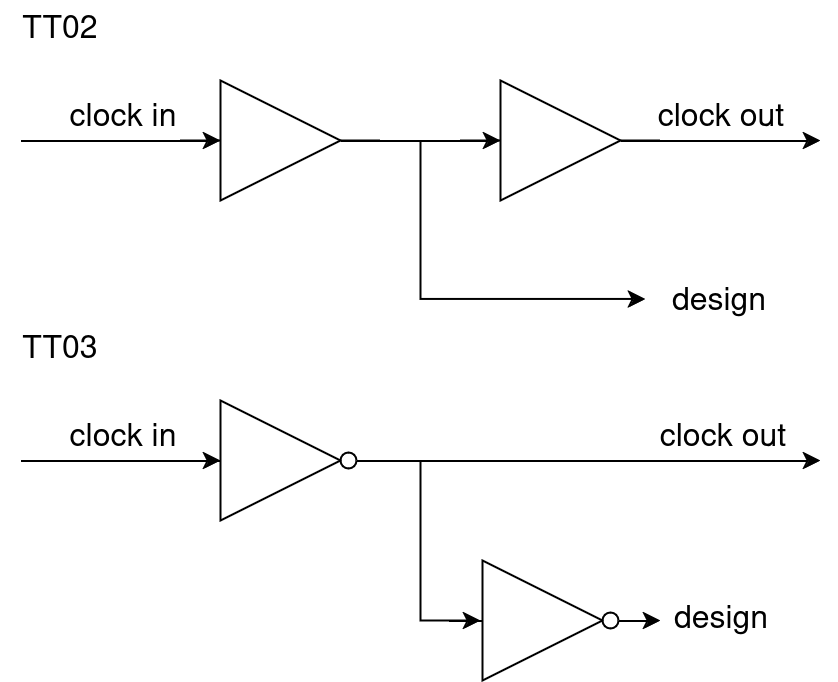
\includegraphics[width=\columnwidth]{./Figs/tt02 vs tt03 scanchain clock.png}
\caption{The Tiny Tapeout 3 architecture buffers the output from the clock network into each design. Clock polarity is alternated between designs to minimize asymmetry between positive and negative cycles.}
\label{fig:TT02_vs_TT03}
\end{figure}

Following the closure of Tiny Tapeout 3, an invitational experimental shuttle dubbed Tiny Tapeout 3.5 ~\cite{tinytapeout03p5} was submitted for production. This featured with 32 designs, testing and previewing some of the changes planned for Tiny Tapeout 4, detailed in the next section. These designs submitted for production in Efabless chipIgnite 2306C.
Two of these designs included a power gate as a stepping stone to supporting analog and mixed signal designs.

%Again, this needs expansion. Maybe each Tiny Tapeout section should start with a paragraph detailing when it opened for submissions, when it closed, how many submissions there were, when and on what shuttle it was sent for manufacture, and when hardware was received (or when it will be received, where it hasn't arrived yet.
